% !TEX root = ../main.tex

\chapter{相干首波}

\section{声速的测量}

任何曾经修学过大学物理实验的本科生都熟悉如何在空气或水这类连续介质中测量声速,即两个声学探头在介质中相对,使用诸如共振波节法、相位法和时差法计算声速。前两者的原理都是寻找固定频率 $f$ 信号的某个特殊相位(如峰值所对应的 $\uppi/2 + 2n\uppi$,$n\in\mathbb{Z}$)下的空间位置,通过逐差法求解声波的波长 $\lambda$,从而根据 $v=f\lambda$ 计算出声速;时差法则是考虑到了声学探头中由于压电陶瓷进行声-电信号转换需要一定的固有时间(当然实际上还有线缆本身传输信号所需要消耗的时间,但是与压电陶瓷的用时相比小得多,在实验时忽略不计),即 $\Delta L = v\times(\Delta t - t_{0})$, 所以通过拟合空间位置与到达时间的斜率 $\mathrm{d}L/\mathrm{d}t$ 以确定声速。

事实上,在颗粒固体中测量声速时,上述几种方法都有着不同程度的应用,如 Paul A.Johnson 和 Xiaoping Jia 同时使用共振法与行波法(即飞行时间法,Time of Flight, T.O.F.)测定颗粒介质中的声速\cite{Johnson_2005};而在地震学中,基于连续小波变换\cite{9356107}(Continuous Wavelet Transform, CWT)和频散能量图(Dispersion Energy Map)求解地震波相速度的方法也被广泛应用。本节将介绍如何将飞行时间法与频散能量图应用于颗粒介质的声速测量中。

\subsection{装置搭建}

目前部署的声学激励与探测系统硬件、软件陈列如下:

\begin{itemize}
  \item Tektronix Arbitrary Function Generator AFG31021。该仪器可以按照实验需求产生如连续正弦波、设定循环数与触发时间间隔的正弦波列、单频脉冲等电压信号,用于激励声学探头产生对应机械振动。其支持写入自定义函数来对信号波形进行控制;
  \item Tektronix TBS2204B 示波器。该示波器通过 BNC 接口对可多达 $4$ 个独立模拟电压信号进行同步采集,可用于同时记录试探信号以及在颗粒介质中传播后的响应信号。该示波器可以调控探头衰减系数($1\times$ 到 $10\times$ 不等),具体实验时需要进行配平;该示波器的采样率最高可达 $1\unit{\giga\hertz}/\unit{Ch}$;单次采样长度最高可达 $5\times 10^{6}$,因此在进行快速傅里叶变换(Fast Fourier Transform,FFT)时,确保我们所关心频域区间的分辨精度足够高。特别的是,示波器具有高精度采集和平均采集等多种采样模式,前者可用于记录瞬时事件信号,而后者则是通过 \numrange{16}{512} 次采集的平均极大地减少了热噪声的影响,从而得到平滑的响应信号。通过 IPv4 网口可使用 TekScope 软件对 TBS2204B 进行数据读取和记录,并且进行简单程度的操控(开始/停止记录)等。而 KickStart 软件能对 AFG31021 与 TBS2204B 进行同步控制,并且能记录多次运行所输入的信号,在实验结束时统一导出,从而极大地便利了对于声学信号的研究;
  \item ATA-101B Power Amplifier。可以设置输入与输出的线缆阻抗(输入端可选取 $50\unit{\ohm}/1\unit{\mega\ohm}$,输出端可选取 $50\unit{\ohm}/1.5\unit{\ohm}$。目前声学常用线缆都是 $50\unit{\ohm}$),其主要功能是以最小步长 $2\unit{\decibel}$ 放大 AFG31021 产生的电压信号,从而满足使声学探头产生声压振幅的需求,通常适用于有限振幅波的非线性传播等实验中。可设定的最大放大效果为 $20\unit{\decibel}$,但是由于其固有的频域放大极限,若初始输入的电压信号本身幅值已经较高,仍然强行设定超出频域放大曲线的增益值会导致放大器输出信号的畸变与失真。因此在设计含 ATA-101B 的实验时,需要综合考虑信号放大器本身的性能上限;
  \item 清诚声发射 G150 与 W800 (成对)声学探头。声学探头在部分研究领域中又被称为换能器(Transducer),意指作为探头核心元件的压电陶瓷既能够将射频线缆传输的模拟电压信号通过电-压效应转换为机械振动的声信号,又能够感应机械振动的幅值强度、通过压-电效应将声信号转换为模拟电压信号,使其能被进一步展开信号处理与分析。G150 和 W800 分别是适用于 $60-400\unit{\kilo\Hz}$ 和 $50-800\unit{\kilo\hertz}$ 频域范围内工作的探头型号,谐振频率分别为 $150\unit{\kilo\hertz}$ 和 $600\unit{\kilo\hertz}$。在具体应当根据实验需求选取合适的一对探头。两个型号的声学探头主体都是 $\varphi 19\unit{\milli\meter}\times 15\unit{\milli\meter}$ 的圆柱体,柱面与底面由 SUS-304 不锈钢材外壳包裹,增强声学探头的屏蔽抗干扰作用;接触面为陶瓷材料,从而激发压缩波;由于两种探头尺寸相同,便于安装于同一颗粒容器中;
  \item 单轴应力圆柱容器。通过 SOLIDWORKS 软件设计,并采用厚度 \numlist{6;8;10}\unit{\milli\meter} 的亚克力板材料制作的容器(采用透明容器是为了兼容未来可能的 X 射线扫描建模需求)。容器内径为 $D = 90\unit{\milli\meter}$, 最高支持厚度为 $13\unit{\centi\meter}$ 的颗粒介质进行实验。设置四柱单轴活塞以及用于放置金属块的加压台,从而对容器内的颗粒介质施加单轴应力,活塞与容器底部中心均留有 $\varphi=19\unit{\milli\meter}$ 的孔洞用于安装声学探头,具体制作时考虑公差为 $0.2\unit{\milli\meter}$。$10\unit{\milli\meter}$ 的亚克力板弯曲为圆筒而制作为容器壁,因此可以安全承担实验需求范围的应力。由于探头本身并非防水型号,因此在设计与制作时容器并未考虑防水/密封处理。
\end{itemize}

%%% 这里放实验装置部件的示意图

%%% 放一个 101B 的频域放大极限的示意图

%%% 找到一个用 tikz 画工作流示意图的方法

需要特别说明的是,一般情况下作用于接收器表面的声压 $p(t)$ 都并不等于入射波的声压 $p_{i}(t)$,这是由探头硬质陶瓷圆面本身存在的声阻抗 $\widetilde{Z}_{S}(\omega)$ 所导致的:

\begin{equation}
  p(t) = \left(1 + \frac{\widetilde{Z}_{S}(\omega)}{\rho_{0}c_{0}S}\right) =\widetilde{K}(\omega)p_{i}(t).
\end{equation}

其中 $\rho_{0}$ 与 $c_{0}$ 是介质处于平衡态时的密度和声速,$S$ 是圆面探测器的面积。接收声压 $p(t)$ 通过非幺正角频率傅里叶变换得到的信号频谱为

\begin{equation}
  F(\omega) = \int_{-\infty}^{+\infty}\widetilde{K}(\omega)p_{i}(t){\ee}^{-\ii\omega t}\mathrm{d}t = \widetilde{K}(\omega)F_{i}(\omega).
\end{equation}

其中 $F_{i}(\omega)$ 为入射波声压 $p_{i}(t)$ 的非幺正角频率傅里叶变换。因此入射波声压 $p_{i}(t)$ 为

\begin{equation}
  p_{i}(t) = \frac{1}{2\uppi}\int_{-\infty}^{+\infty}\frac{F(\omega)}{\widetilde{K}(\omega)}{\ee}^{\ii\omega t}\mathrm{d}\omega\label{eq:response_correct}
\end{equation}

在实验中,由于我们使用的是一对同工作频域的探头,面对面接触时可以简单视为声波经历了两次同样的声阻抗过程,且假定实验工作范围内使用的模拟电压信号幅值产生的压电效应满足线性($p\propto U$)。那么,我们可以设定信号发生器产生的电压信号为 $U_{0}(\omega)$,则接收到的电压信号为

\begin{equation}
  U(\omega) = \widetilde{K}(\omega)^{2}U_{0}(\omega).
\end{equation}

为了测定探头的声阻抗,我们可以使用连续正弦电压信号对探头进行激励,并且将其理解为受迫阻尼振动过程:

\begin{equation}
  \frac{\mathrm{d}^{2}x}{\mathrm{d}t^{2}} + 2\beta\frac{\mathrm{d}x}{\mathrm{d}t} + \omega_{0}^{2}x = f\cos{\omega t},
\end{equation}

观察受迫振动的稳态解,即取 $t\rightarrow \infty$ 极限:

\begin{equation}
  \lim_{t\rightarrow \infty} x(t) = \frac{f}{\sqrt{(\omega_{0}^{2} - \omega^{2})^{2} + 4\beta^{2}\omega^{2}}}\cos{(\omega t - \phi)},\quad \phi = \arctan{\left(\frac{2\beta\omega}{\omega_{0}^{2}-\omega^{2}}\right)}
\end{equation}

即激励信号源的振幅和响应信号振幅呈现线性,因此我们可以使用源信号振幅作为分母来对响应效率函数进行重标定。图~\ref{fig:response_factor} 展示了设定源信号为一系列相同振幅 $U = 1\unit{Vpp}$、不同频率 $\omega_{n}$ 的连续正弦波列 $\{U(\omega_{n})\}$ 对探头进行激励,示波器的探头衰减系数均设定为 $1\times $ 时所测定的探头响应系数 $\widetilde{K}(\omega)$。

\begin{figure}[!htp]
  \centering
  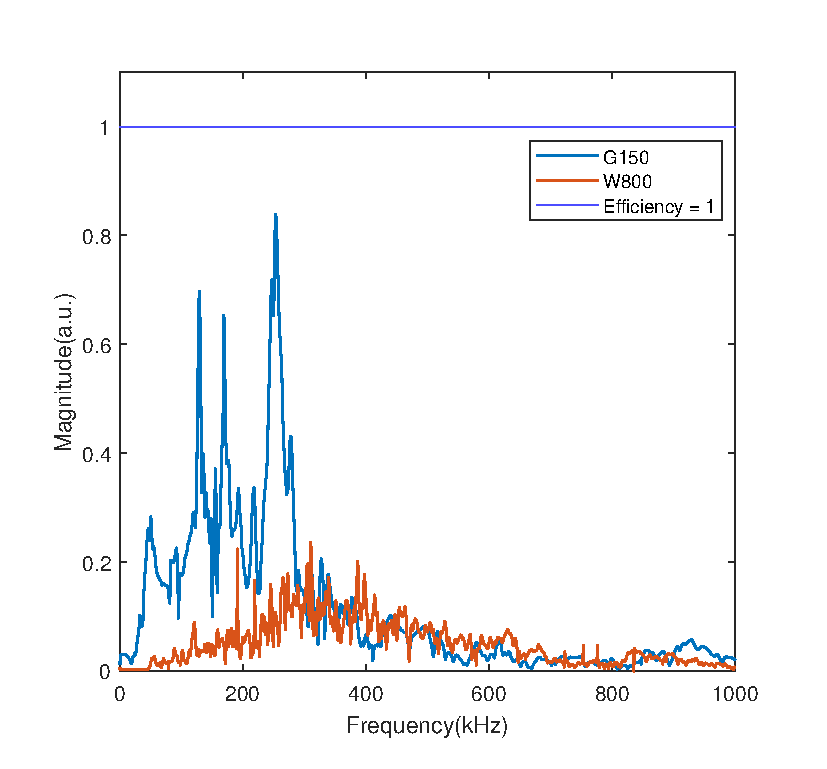
\includegraphics[height=8cm]{2_response_factor.eps}
  \bicaption{G150 与 W800 两种声学探头响应系数 $\widetilde{K}(\omega)$}{Response factor $\widetilde{K}(\omega)$ of G150 and W800 acoustic sensors}
  \label{fig:response_factor}
\end{figure}

观察可知,G150 在 \numrange{60}{400}\unit{\kilo\hertz} 频域内的响应系数较高,在某些频率下甚至非常接近 $1$, 而超出其工作频域的响应系数迅速跌落;而 W800 虽然在我们所关心的频域,即 \numrange{0}{1000}\unit{\kilo\hertz} 内响应系数均不高,但是胜在响应曲线相对平稳。因此在实验时,如果信号集中于超声频域内的较低成分($\leq 400\unit{\kilo\hertz}$),那么选择 G150 将是更合理的;在关心较广的频域下的声学参数(比如衰减、相速度等)时,W800 的性能相对优异。为了弥补 W800 本身响应系数较低的缺陷,未来可以考虑使用 Physics of Acoustic Company 的 2/4/6 Type 等型号的供电前置放大器来对响应信号进行增强,从而增加信噪比、便于实验后续的信号提取与分析。

我们后续实验便可以借助式~\eqref{eq:response_correct} 来对实验中采集的响应信号进行修正。需要说明的是,声阻抗系数本身是复数,即探头本身对于信号会产生相位上的影响,但是如何准确测定这种相位差并且进行有效插值是一个较为困难的问题。因此在实际实验时,对于时间/相位相关的实验我们并不使用上述的修正方法,而是直接使用原始信号分析。

\subsection{飞行时间法测定颗粒介质中的声速}

飞行时间法,在部分文献与研究工作中又被称为行波法,其测定声速的原理即测量试探声波从声源探头传播到接收探头所消耗的时间长度 $\Delta t$,从而计算得到

\begin{equation}
  V_{\text{T.O.F.}} = \frac{L}{\Delta t},\quad \Delta t = t_{A} - t_{G}.
\end{equation}

其中 $L$ 是两个探头之间颗粒介质的厚度。但具体到实际数据处理操作中,由于响应信号本身是一个多频率成分、多峰值、在时间上具有一定长度的波列,所以如何准确定义传输声波的到达时间 $t_{A}$(A = Arrival)是值得商榷的问题。为了研究这个细节,Ellák Somfai 等人定义了颗粒介质中声波的三种不同的到达时间:波前到达时间 $t_{0}$(由于热噪声的干扰作用,波前通常被定义为信号的首个上升沿峰值 $A_{1}$ 的 $10\%$ 处而与噪声幅值区分开,部分更激进的研究者会选取为 $3\%$),(首个)波峰到达时间 $t_{1}$,首次过零时间 $t_{2}$\cite{PhysRevE.72.021301}。良好定义的波速应当满足在不同厚度下测得的结果相近,因此我们可以按照其确定在使用飞行时间法测定声速时的最佳信号参考点。

%%% 这里放参考文献的三个不同到达时间的示意图

\subsubsection{信号最佳参考点选取}

我们在实验中使用 Tektronix 示波器对源信号与响应信号进行了同步采集,因此容易确定具体的时间起点。下面我们简单介绍有关于如何识别信号得到各定义下的到达时间的算法。

首先我们需要测量探头本身通过压电效应进行信号转换所需要的固有耗时,这里我们采用的是 face-to-face time 的测量方法,即测量两个探头的陶瓷探测圆面直接紧密接触所时,声波传播所需要的耗时。

\begin{enumerate}
  \item 信号平滑。由于示波器的采样频率通常很高,而且存在着一定的热噪声对信号进行干扰,因此我们借助 Matlab 的 movmean() 函数对信号进行线性权重的平滑处理。我们通过平均窗口长度 $num_window$ 来控制平滑程度,该量既不能过小,使得热噪声未能被充分处理,也不能过大使得真正的响应信号也被模糊失真;
  \item 识别源信号(Src. = Source)的首峰时刻。作为源振幅信号,其信噪比明显很高,因此我们可以使用较大的噪声阈值,如源信号振幅的 $40\%$,通过 findpeaks() 函数识别源信号的首个峰值。源信号的峰值位置识别通常准确率很高。需要注意的是,即使在采集时已经在示波器上设定源振幅信号和响应信号的偏置值为 $0\unit{V}$,由于系统硬件本身的问题仍然会导致源信号和响应信号存在一定量的偏置值,而这会对后续识别信号的波前位置造成影响。
  \item 计算源信号的偏置值。取首峰幅值的 $1/80$ 作为其波前定义,通过 find() 函数找到其对应的时刻 $t_{O}$,即近似为源信号的发射时刻。取所记录的源信号中发射时刻前的信号均值作为源信号的偏置值,并将源信号减去该偏置值作为修正。由于在记录信号时已经使用了 $128$ 次平均采集,所以热噪声造成的幅值涨落已经被尽可能消除,因此计算所得到的偏置值是相对准确的。
  \item 识别响应信号(Res. = Response)的首峰时刻。从该步骤开始,需要通过控制寻峰算法中的 findpeaks() 函数中的峰最小半高宽(MinPeakWidth)和噪声阈值(MinPeakProminence),并且需要通过。
\end{enumerate}

图~\ref{fig:reference_point}是对典型的响应信号进行三种不同到达时间识别的实例。


\begin{figure}[!htp]
  \centering
  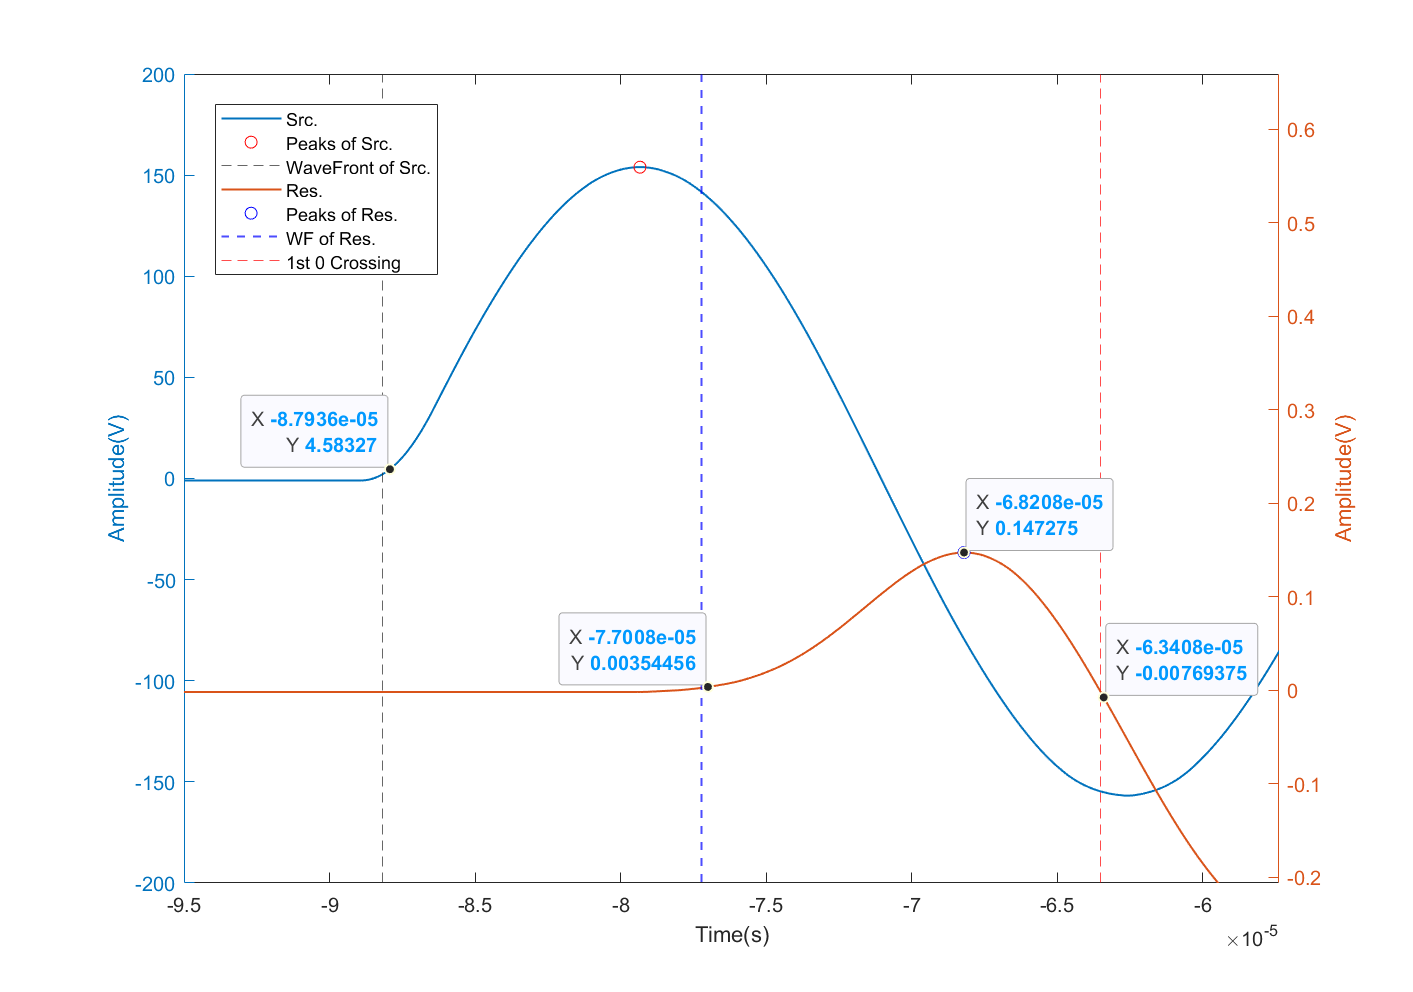
\includegraphics[height=8cm]{2_reference_point.png}
  \bicaption{同步采集源信号与响应信号,以及波前到达时刻,波峰到达时刻与首次过零时刻}{Synchronized acquisition of source and response signals, as well as wavefront arrival, peak arrival and first zero crossing moments}
  \label{fig:reference_point}
\end{figure}

我们按照上述三种到达时间的识别方法,测定了在不同厚度下的声速。特别地,我们额外使用时差法拟合得到了声速 $V_{L}$,并将其与飞行时间法测定的声速 $V_{\text{T.O.F.}}$ 进行比较。结果如图~\ref{fig:sound_velocity_measurement} 所示。实验中所使用的颗粒为 $d=2\unit{\milli\meter}$ 的钢珠,施加的单轴应力为 $P=9\unit{\kilo\Pa}$,试探信号设定为 $5$ 循环 $30\unit{\kilo\Hz}$ 正弦波列。为了尽可能消除颗粒介质本身随机性的误差,每一个厚度都需要重新制备 $7$ 个独立不同的随机密堆积以进行到达时间的系综平均,即 $t_{i}\rightarrow \bar{t}_{i}$。

\begin{figure}[!hbtp]
  \centering
  \bisubcaptionbox{以三种参考点通过时差法求得的声速 $V_{L}$}%
                  {Sound velocity $V_{L}$ measured by time difference method with three reference points}%
                  [6cm]{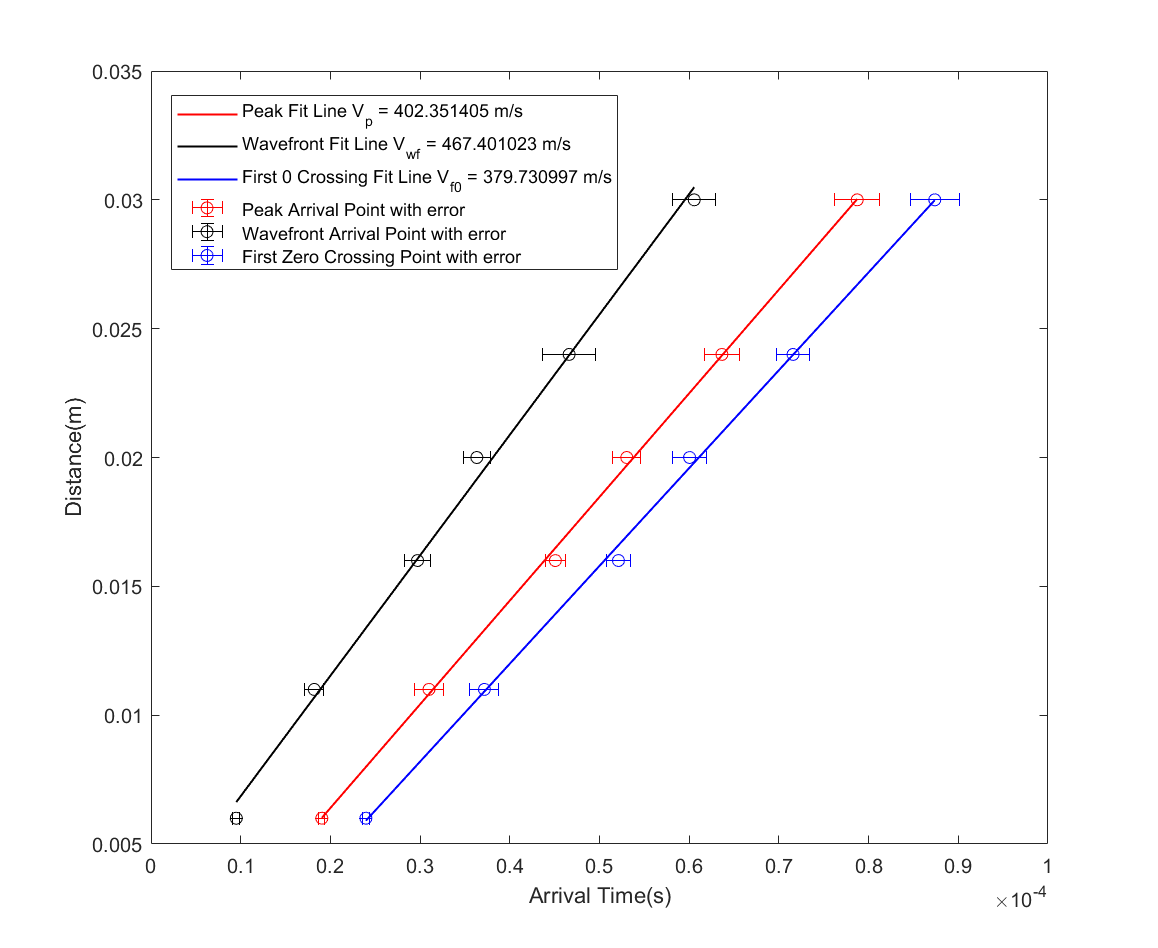
\includegraphics[height=6cm]{2_fitted_velocity.png}}
  \hspace{1cm}
  \bisubcaptionbox{以三种参考点通过飞行时间法求得的声速 $V_{\text{T.O.F.}}$}%
                  {Sound velocity $V_{\text{T.O.F.}}$ measured by Time of Flight method with three reference points}%
                  [6cm]{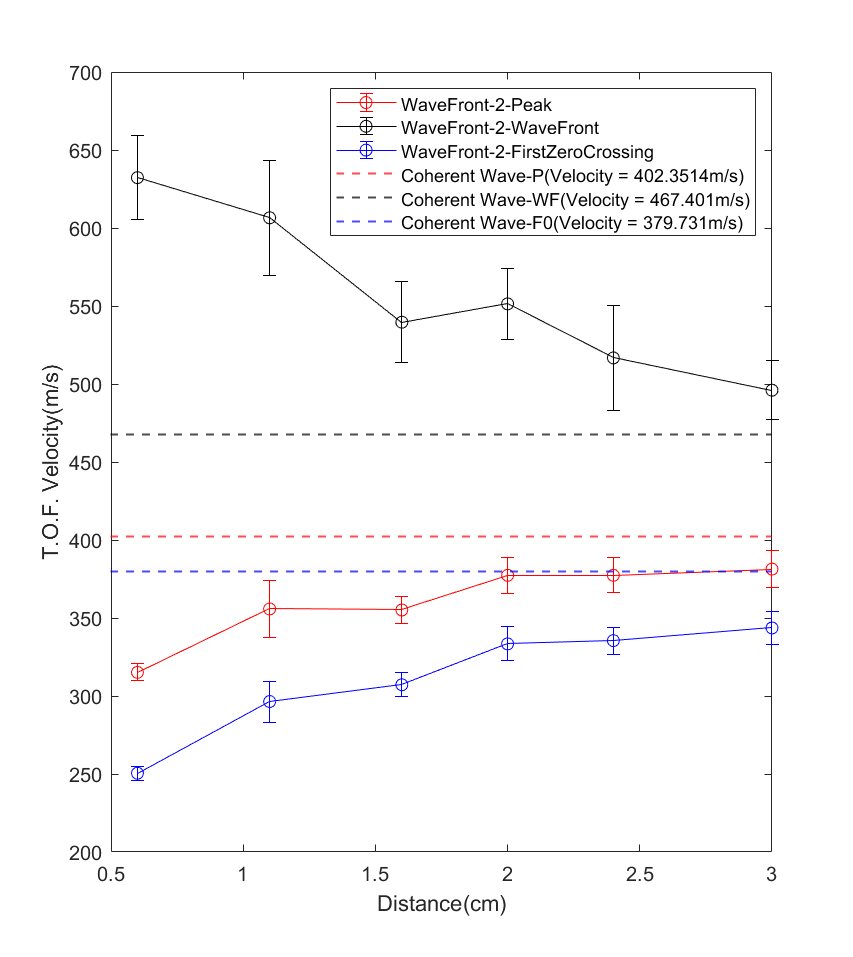
\includegraphics[height=6cm]{2_tof_velocity_and_fitted_velocity.png}}
  \bicaption{$5$ 循环 $30$ 千赫兹正弦波列作为试探信号,颗粒介质为直径 $2$ 毫米钢珠的随机密堆积,单轴应力 $9$ 千帕下的声速测量}
            {Velocity of sound measurements at $9\unit{\kilo\Pa}$ uniaxial stress with $5$-cycle of a $30\unit{\kilo\Hz}$ sine wave train as a test signal and a randomized stack of $2\unit{\milli\meter}$ diameter steel beads as the granular medium}
  \label{fig:sound_velocity_measurement}
\end{figure}

由此可见,各参考点的飞行时间法定义下的声速随着传播距离 $L$ 的增大向各自的时差法定义下的声速 $V_{L}$ 逼近,其中以波峰到达时间 $t_{1}$ 定义的声速在距离上的变化最为稳定。因此在传播距离 $L$ 充分大时,我们可以使用飞行时间法替代时差法进行工程上的声速测量(因为时差法需要改变探头间的距离,而有的实验并不允许改变这一点,如与颗粒堆积结构本身相关的可逆性研究\cite{PhysRevE.84.020301}),而其中以波峰到达时间 $t_{1}$ 定义的又是最好的。

需要额外说明的是,这三种定义的参考点对于时差法都可以适用,但是其拟合计算出的声速大小的顺序与各参考点的在时间上的先后顺序明显相关(即参考点随着传播时间/距离的增大出现了逐渐分离的现象),我们将其概括为相干首波在颗粒介质中随着传播距离增大而出现的展宽。这意味着至少在频域的速度分布上颗粒介质已经表现出了异质性,即出现了色散现象;我们将在后文通过设计描述首波峰展宽程度的归一化宽度 $W$ 以及相关实验从而更详细地探讨这一点。

% \begin{figure}[!hbtp]
%   \centering
%   \subcaptionbox{健康/损伤信号}%
%                 [7cm]{\includegraphics[height=6cm]{figures/signal_1.png}}
%   \hspace{1cm}
%   \subcaptionbox{散射信号}%
%                 [7cm]{\includegraphics[height=6cm]{figures/signal_2.png}}
%   \caption{响应信号处理}
%   \label{fig:bisubcaptionbox}
% \end{figure}

\subsection{频散能量图法}

\subsubsection{测量相速度的原理推导}

考虑单频连续正弦波作为声源激励,如果我们将颗粒介质中的声学传播简单考虑为单频平面波,即

\begin{equation}
  s(x,t) = A_{0}{\ee}^{-\alpha x}{\ee}^{\ii(\omega x/V_{\varphi}-\omega t)},
  \label{eq:spherical_wave}
\end{equation}

其中 $A_{0}$ 是声源振幅,$\alpha$ 描述声信号在颗粒介质中随着传播距离 $x$ 的衰减系数,$V_{\varphi}$ 是信号角频率为 $\omega$ 时的相速度。假定在距离声源 $x_{1}$ 与 $x_{2}$ 处存在两个小接收探头(即忽略可能造成的反射),分别接收到声波信号 $S_{1}(t)$ 与 $S_{2}(t)$。则能求解相速度为

\begin{equation}
  V_{\varphi} = \frac{x_{2}-x_{1}}{\Delta \varphi}\omega.
\end{equation}

我们很容易想到通过 FFT 算法求解两次信号的相位频谱 $\varphi_{i}(\omega)$, 但是显然

\begin{equation}
  \Delta \varphi = \varphi_{2}(\omega) - \varphi_{1}(\omega) + 2N(\omega)\uppi
\end{equation}

对于 $N(\omega)$ 的确定则较为困难,因此地震学提出使用频散能量图观察相速度可能的分布情况。引入信号 $S_{i}(t)$ 与 $S_{j}(t)$ 的互关联函数 $C_{i,j}(\tau)$:

\begin{equation}
  C_{i,j}(\tau) = \int_{-\infty}^{+\infty}S_{i}(t)S_{j}(t+\tau)\mathrm{d}t.
\end{equation}

其中 $\tau$ 是描述信号延迟/传播时间的参数,因此该函数是一个时域函数。对其进行非幺正角频率傅里叶变换:

\begin{align}
  \mathcal{F}[C_{1,2}(\tau)] &= \int_{-\infty}^{+\infty}{\ee}^{-\ii\omega\tau}\int_{-\infty}^{+\infty}S_{1}(t)S_{2}(t+\tau)\mathrm{d}t\mathrm{d}\tau \nonumber \\
  &= \int_{-\infty}^{+\infty}S_{1}(t)\int_{-\infty}^{+\infty}{\ee}^{-\ii\omega\tau}S_{2}(t+\tau)\mathrm{d}\tau\mathrm{d}t \nonumber \\
  &= \int_{-\infty}^{+\infty}S_{1}(t)S_{2}(\omega){\ee}^{\ii\omega t}\mathrm{d}t \nonumber \\
  &= S_{1}^{*}(\omega)S_{2}(\omega).
\end{align}

其中 $S_{1}^{*}(\omega)$ 和 $S_{2}(\omega)$ 分别是 $S_{1}(t)$ 和 $S_{2}(t)$ 的非幺正角频率傅里叶变换计算而来的频谱,上标 $^{*}$ 表示取该复数量的共轭。接下来通过狄拉克函数 $\delta(\omega-\omega_{n})$ 提取角频率为 $\omega_{n}$ 信号分量的延迟时间 $\tau_{n}$ 的信息,再对其进行逆非幺正角频率傅里叶变换:

\begin{align}
  \mathcal{F}^{-1}\left\{\delta(\omega-\omega_{n})\mathcal{F}[C_{1,2}(\tau)]\right\} &= \frac{1}{2\uppi}\int_{-\infty}^{+\infty}S_{1}^{*}(\omega)S_{2}(\omega)\delta(\omega_{n}){\ee}^{\ii\omega\tau}\mathrm{d}\omega \nonumber \\
  &= \frac{1}{2\uppi}S_{1}^{*}(\omega_{n})S_{2}(\omega_{n}){\ee}^{\ii\omega_{n}\tau}.
\end{align}

具体绘制二维概率分布时,我们只需以 $S_{1}^{*}(\omega_{n})S_{2}(\omega_{n}){\ee}^{\ii\omega_{n}\tau}/2\uppi$ 的最大值进行归一化,并且取计算后的实部即可。该函数的物理含义是,延迟时间为 $\tau$ 时,即该频率分量 $\omega_{n}$ 对应的相速度为 $V_{\varphi} = \Delta x/\tau$ 的可能性大小(得到的将是 $[-1,1]$ 之间的数值,即越接近 $1$ 可能性越高)。通过设置离散频率分布 $\{\omega_{n}\}$, 即可查看在颗粒介质中可能的相速度分布。需要说明的是,频散能量图没有从根本上解决 $N(\omega)$ 的确定问题,但是为辅助飞行时间法测定声速提供了更直观的参考工具。

\subsubsection{颗粒介质中相速度分布}


\begin{figure}[!hbtp]
  \centering
  \bisubcaptionbox{在 $x_1=1.1\unit{cm}$ 与 $x_{2}=2.0\unit{cm}$ 处采集的响应信号}{Reponse signal captured at $x_1=1.1\unit{cm}$ and $x_{2}=2.0\unit{cm}$}%
                [7cm]{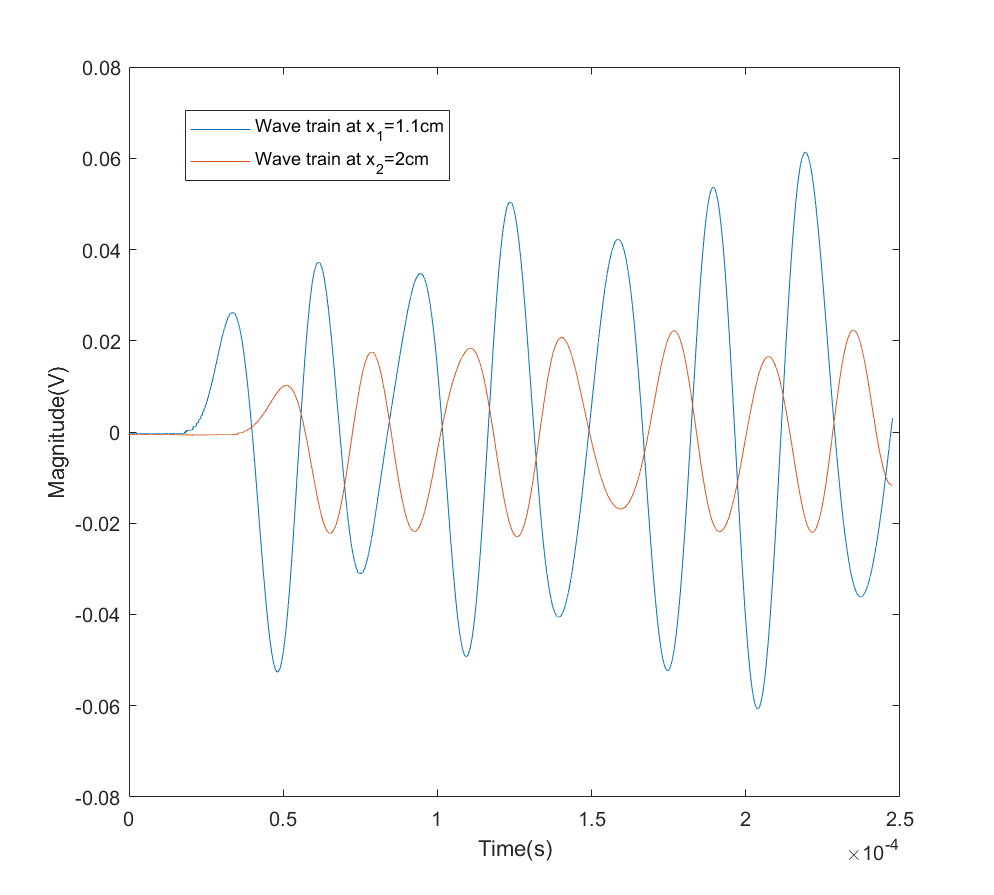
\includegraphics[height=6cm]{figures/2_wave_train.png}}
  \hspace{1cm}
  \bisubcaptionbox{$0-60\unit{kHz}$ 的相速度频域分布热图}{Phase velocity frequency distribution heat map at $0-60\unit{kHz}$}%
                [7cm]{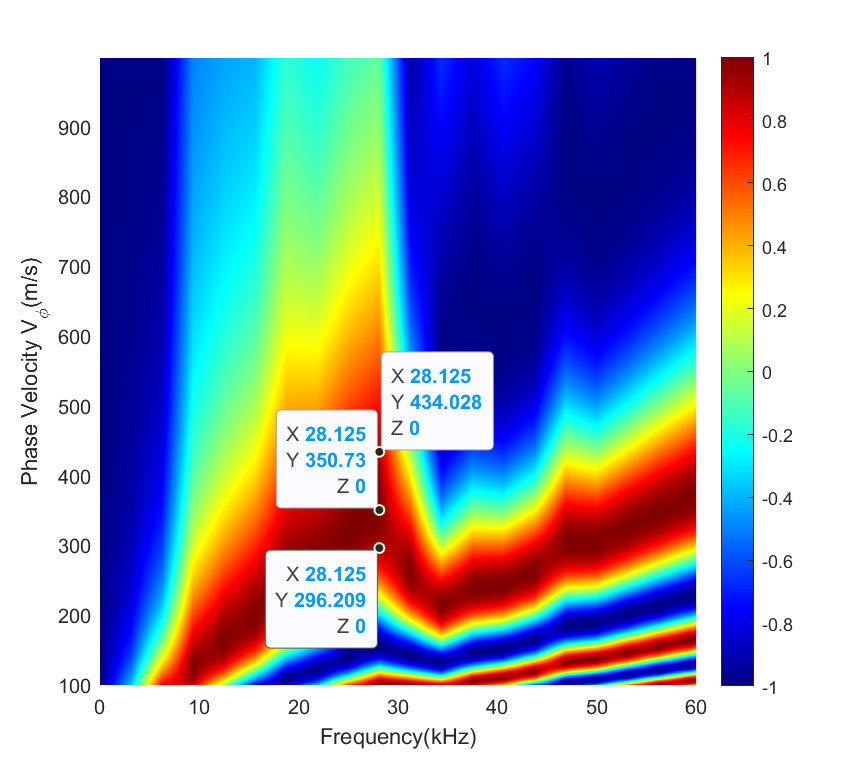
\includegraphics[height=6cm]{figures/2_cwt_v_phi.png}}
  \bicaption{根据异地响应信号计算频散能量图}{Dispersion energy map calculated from separated response signals}
  \label{fig:dispersion_energy}
\end{figure}

图 \ref{fig:dispersion_energy} 展示了在单轴应力容器中,根据不同采集距离 $x_{1}$、$x_{2}$ 下的两道压缩波信号绘制的频散能量图。可以看到两道信号在发射信号的中心频率 $f_{c} = 30\text{ kHz}$ 处的相速度约为 $V_{\varphi} = 350\pm 10\unit{m/s}$。

\section{声速与单轴应力的指数关系}

\subsection{等效介质理论(EMT)}

假定声波波长 $\lambda\gg$ 颗粒直径 $d$,颗粒体系由相同颗粒组成,满足紧束缚条件,颗粒介质应变可采用仿射近似,则纵波声速 $V_{L}$ 与横波声速 $V_{T}$ 分别为

\begin{align}
  V_{L} &= \sqrt{\frac{(K+\frac{4}{3}G)}{\rho^{*}}},\label{eq:emt_velocity_L},\\
  V_{T} &= \sqrt{\frac{G}{\rho^{*}}}.\label{eq:emt_velocity_T}
\end{align}

其中 $K$ 与 $G$ 分别是颗粒介质的体弹性模量与剪切弹性模量,$\rho^{*}=\rho\phi$ 是颗粒固体的密度,$\rho$ 是颗粒材料的密度,$\phi$ 是颗粒介质的体积分数。在 EMT 中两个模量通过以下式子给出:

\begin{align}
  K &= \frac{C_{n}}{12\uppi}\left(\phi Z\right)^{\frac{2}{3}}\left(\frac{6\uppi P}{C_{n}}\right)^{\frac{1}{3}},\\
  G &= \frac{C_{n} + \frac{3}{2}C_{t}}{20\uppi}\left(\phi Z\right)^{\frac{2}{3}}\left(\frac{6\uppi P}{C_{n}}\right)^{\frac{1}{3}},
\end{align}

其中 $Z$ 是颗粒的平均接触数,$C_{n}$、$C_{t}$ 分别是描述颗粒在法向和切向与力相关的系数。Hertz 接触模型和 Mindlin 接触模型分别使用了这两个系数,即两个颗粒通过接触完成的相互作用力为

\begin{align}
  f_{n} &= \frac{2}{3}C_{n}R^{\frac{1}{2}}w^{\frac{3}{2}},\\
  f_{t} &= C_{t}(Rw)^{\frac{1}{2}}\Delta s,
\end{align}

其中 $w$ 是半径分别为 $R_{1}$、$R_{2}$ 的两个颗粒之间的重叠量,$R = \frac{2R_{1}R_{2}}{R_{1} + R_{2}}$ 为颗粒的等效半径。引入颗粒组成材料(下标 $g$)的剪切模量 $G_{g}$ 与泊松比 $\nu_{g}$,完成对力系数的表述:

\begin{align}
  C_{n} &= \frac{4G_{g}}{1-\nu_{g}},\\
  C_{t} &= \frac{8G_{g}}{2-\nu_{g}}.
\end{align}

现在我们从颗粒体系的应力-应变角度出发,通过假定颗粒介质具有各向同性,以及前文所提到的仿射近似条件下,求得颗粒介质模量\cite{WALTON1987213}。假定颗粒介质中两相邻接触的颗粒坐标分别为 $\mathbf{r}^{(m)}$、$\mathbf{r}^{(n)}$,且颗粒球体的半径为 $R$。那么从颗粒 $m$ 指向颗粒 $n$ 的相对坐标位矢的单位矢量为

\begin{equation}
  \mathbf{I}^{(nm)} = \frac{\mathbf{r}^{(n)} - \mathbf{r}^{(m)}}{2R}\label{eq:unit_vector}
\end{equation}

标记两颗粒的空间位移量分别为 $\mathbf{u}^{(m)}$、$\mathbf{u}^{(n)}$,借助式~\eqref{eq:unit_vector} 可以提取出两颗粒相对位移在其接触面法向与切向的分量,而这正是 Hertz 接触与 Mindlin 接触中所需要的法向与切向形变信息:

\begin{align}
  w_{0} &= \frac{\mathbf{u}^{(m)} - \mathbf{u}^{(n)}}{2}\cdot \mathbf{I}^{(nm)},\\
  \Delta s &= \frac{\mathbf{u}^{(m)} - \mathbf{u}^{(n)}}{2} - w_{0}\mathbf{I}^{(nm)} = \frac{\mathbf{u}^{(m)} - \mathbf{u}^{(n)}}{2} - \left[\frac{\mathbf{u}^{(m)} - \mathbf{u}^{(n)}}{2}\cdot \mathbf{I}^{(nm)}\right]\mathbf{I}^{(nm)}.
\end{align}

注意这里所取的上标,使得法向形变量指向颗粒体心之外。代入各形变量到对应的接触力模型中,我们可以计算两颗粒之间通过接触产生的相互作用力:

\begin{equation}
  \begin{aligned}
  \mathbf{F}^{(nm)} &= \mathbf{F}_{N}^{(nm)} + \mathbf{F}_{T}^{(nm)}\\
  &= \frac{4R^{\frac{1}{2}}w_{0}^{\frac{3}{2}}}{3\uppi B}\mathbf{I}^{(nm)} + \frac{8(Rw_{0})^{\frac{1}{2}}}{3\pi(2B+C)}\left[\frac{\mathbf{u}^{(m)} - \mathbf{u}^{(n)}}{2} - w_{0}\mathbf{I}^{(nm)}\right]\\
  &= \frac{(2R)^{\frac{1}{2}}}{3\uppi B(2B+C)}\left\{2B\left[\left(\mathbf{u}^{(n)} - \mathbf{u}^{(n)}\right)\cdot \mathbf{I}^{(nm)}\right]^{\frac{1}{2}}\left(\mathbf{u}^{(m)} - \mathbf{u}^{(n)}\right)\right.\\
   &+ \left.C\left[\left(\mathbf{u}^{(m)} - \mathbf{u}^{(n)}\right)\cdot \mathbf{I}^{(nm)}\right]^{\frac{3}{2}}\mathbf{I}^{(nm)}\right\}
  \end{aligned}\label{eq:contact_force}
\end{equation}

其中

\begin{align}
  B &= \frac{1}{4\uppi}\left(\frac{1}{\mu} + \frac{1}{\lambda + \mu}\right),\\
  C &= \frac{1}{4\uppi}\left(\frac{1}{\mu} - \frac{1}{\lambda + \mu}\right),
\end{align}

而 $\lambda$ 和 $\mu$ 是颗粒材料的 Lamé 系数。假设颗粒的形变与样品的应变满足

\begin{equation}
  {u}_{i}^{(n)} = \mathbf{e}_{ij}{r}_{j}^{(n)}\label{eq:strain_displacement},
\end{equation}

其中 $\mathbf{e}_{ij}$ 是描述颗粒介质应变的张量,${r}_{j}^{(n)}$ 是颗粒 $n$ 在 $j$ 轴上的位矢分量,${u}_{i}^{(n)}$ 是颗粒 $n$ 在 $i$ 轴上的位移分量。这里使用类似于 Einstein 求和约定的写法而省略了等号右边原本应有的 $\sum_{j}^{x,y,z}$ 求和符号。代入式~\eqref{eq:unit_vector}、\eqref{eq:strain_displacement}至式~\eqref{eq:contact_force} 中,从而有

\begin{equation}
  F_{i}^{(nm)} = -\frac{4R^{2}}{3\uppi B(2B+C)}\left\{2B\left(-e_{i^{\prime}j^{\prime}}\mathbf{I}_{i^{\prime}}^{(nm)}\mathbf{I}_{j^{\prime}}^{(nm)}\right)^{\frac{1}{2}}e_{ij}\mathbf{I}_{j}^{(nm)} - C\left(-e_{i^{\prime}j^{\prime}}\mathbf{I}^{(nm)}_{i^{\prime}}\mathbf{I}_{j^{\prime}}^{(nm)}\right)^{\frac{3}{2}}\mathbf{I}_{i}^{(nm)}\right\}.
\end{equation}

接下来我们尝试描述颗粒介质中的应力-应变关系。颗粒介质的平均应力可以表示为颗粒间相互作用的矢量和平均,即

\begin{equation}
  \langle\sigma_{ij}\rangle = \frac{1}{V}\int\sigma_{ij}\mathrm{d}V = \frac{1}{V}\sum_{n}\int\sigma_{ij}^{(n)}\mathrm{d}V_{n}.
\end{equation}

其中 $V$ 是颗粒介质的体积,$\sigma_{ij}$ 表示在颗粒介质中的 Cauchy 应力,$\sigma_{ij}^{(n)}$ 和 $V_{n}$ 分别表示颗粒 $n$ 的 Cauchy 应力与体积。考虑体积微元 $\mathrm{d}V = \mathrm{d}r\mathrm{d}S$,即有

\begin{equation}
  \int\sigma_{ij}^{(n)}\mathrm{d}V_{n} = \frac{1}{2}\int\left(r_{i}^{\prime}t_{j}^{(n)} + r_{j}^{\prime}t_{i}^{(n)}\right)\mathrm{d}S_{n},
\end{equation}

其中 $\mathbf{r}^{\prime} = \mathbf{r} - \mathbf{r}^{(n)} $ 是颗粒 $n$ 体心指向颗粒间接触点的位矢,而 $\mathbf{t}^{(n)}$ 描述了颗粒 $n$ 的表面 $S_{n}$ 在 $\mathbf{r}$ 处的作用力强度。显然,由于颗粒本身是离散存在的,因此能与颗粒 $n$ 产生接触并且能真正产生作用力的颗粒 $m$ 也是有界的。所以将积分形式转换为求和形式,并使用 $\mathbf{r}^{\prime} = \left(\mathbf{r}^{(m)} - \mathbf{r}^{(n)}\right)/2$,得到

\begin{equation}
  \int\sigma_{ij}^{(n)}\mathrm{d}V_{n} = \frac{1}{2}\sum_{m}\left\{\frac{1}{2}\left(r_{i}^{(m)} - r_{i}^{(n)}\right)F_{j}^{(nm)} + \frac{1}{2}\left(r_{j}^{(m)} - r_{j}^{(n)}\right)F_{i}^{(nm)}\right\}\label{eq:cauchy_tensor}.
\end{equation}

代入~\eqref{eq:unit_vector} 于式~\eqref{eq:cauchy_tensor},得到

\begin{equation}
  \langle\sigma_{ij}\rangle = \frac{R}{V}\sum_{n,m}\left(I_{i}^{(nm)}F_{j}^{(nm)} + I_{j}^{(nm)}F_{i}^{(nm)}\right)\label{eq:cauchy_tensor_2}.
\end{equation}

因为求和符号已经写作 $\sum_{m,n}$ 形式,在式~\eqref{eq:cauchy_tensor} 中用于消除重复计数的系数 $\frac{1}{2}$ 便不再使用。现在我们已经得出了描述力 $F_{i}^{(nm)}$ 的式~\eqref{eq:contact_force},将其代入至~\eqref{eq:cauchy_tensor_2},得到

\begin{equation}
  \begin{aligned}
    \langle\sigma_{ij}\rangle &= \frac{8R^{3}}{3\uppi VB(2B+C)}\sum_{n,m}\left\{B\left(-e_{i^{\prime}j^{\prime}}I_{i^{\prime}}^{(nm)}I_{j^{\prime}}^{(nm)}\right)^{\frac{1}{2}}\left[e_{ik}I_{k}^{(nm)}I_{j}^{(nm)} + e_{jk}I_{k}^{(nm)}I_{i}^{(nm)}\right]\right.\\
    &-\left. C\left(-e_{i^{\prime}j^{\prime}}I_{i^{\prime}}^{(nm)}I_{j^{\prime}}^{(nm)}\right)^{\frac{3}{2}}I_{i}^{(nm)}I_{j}^{(nm)}\right\}
  \end{aligned}\label{eq:cauchy_tensor_3}.
\end{equation}

回顾前面 EMT 的求和假设:颗粒介质呈现几何学上统计性质的各向同性,各颗粒被均匀配位(接触点在球面上均匀分布),颗粒介质的体积足够大,且其中包含充分多的颗粒。所以式~\eqref{eq:cauchy_tensor_3} 可简化为

\begin{equation}
  \begin{aligned}
  \langle\sigma_{ij}\rangle &= \frac{4R^{3}ZN}{3\uppi VB(2B+C)}\left\{B\left\langle(-e_{i^{\prime}j^{\prime}}I_{i^{\prime}}I_{j^{\prime}})^{\frac{1}{2}}(e_{ik}I_{k}I_{j} + e_{jk}I_{k}I_{i})\right\rangle\right.\\
  &-\left.C\left\langle(-e_{i^{\prime}j^{\prime}}I_{i^{\prime}}I_{j^{\prime}})^{\frac{3}{2}}I_{i}I_{j}\right\rangle\right\}.
  \end{aligned}\label{eq:cauchy_tensor_4}
\end{equation}

其中 $Z$ 是各颗粒的平均配位数,$N$ 表示介质中颗粒的总数。引入体积分数

\begin{equation}
  \phi = \frac{N}{V}\frac{4}{3}\uppi R^3
\end{equation}

以化简式~\eqref{eq:cauchy_tensor_4},得到

\begin{equation}
  \begin{aligned}
    \langle\sigma_{ij}\rangle &= \frac{\phi Z}{\uppi^{2}B(2B+C)}\left\{B\left\langle(-e_{i^{\prime}j^{\prime}}I_{i^{\prime}}I_{j^{\prime}})^{\frac{1}{2}}(e_{ik}I_{k}I_{j} + e_{jk}I_{k}I_{i})\right\rangle - C\left\langle(-e_{i^{\prime}j^{\prime}}I_{i^{\prime}}I_{j^{\prime}})^{\frac{3}{2}}I_{i}I_{j}\right\rangle\right\}.
  \end{aligned}\label{eq:cauchy_tensor_end}
\end{equation}

对颗粒介质采取等静压假设(isostatic),即应变在颗粒介质中是均匀的:

\begin{equation}
  e_{ij} = e\delta_{ij},
\end{equation}

这是因为真实的颗粒介质中很难测得一个具体的应变分布。于是化简得到

\begin{equation}
  \langle\sigma_{ij}\rangle = -\frac{\phi Z(-e)^{\frac{3}{2}}}{\uppi^{2}B}\langle I_{i}I_{j}\rangle.\label{eq:expected_value}
\end{equation}

而对于相对坐标的单位矢量 $I$,有 $\langle I_{i}I_{j}\rangle = \frac{1}{3}\delta_{ij}$。约定 $\langle\sigma_{ij}\rangle = -p\delta_{ij}$,即

\begin{equation}
  p = \frac{\phi Z(-e)^{3/2}}{3\uppi^{2}B}.
\end{equation}

这里 $p$ 实际上就是颗粒介质所受的约束应力(confining pressure)。反解出

\begin{equation}
  e = -\left(\frac{3\uppi^{2}Bp}{\phi Z}\right)^{\frac{2}{3}}
\end{equation}

接下来我们尝试求解 EMT 假设下的颗粒介质的等效模量(effective moduli)。弹性模量通过下式给出定义:

\begin{equation}
  \langle\delta\sigma_{ij}\rangle = C_{ijkl}^{*}\langle\delta e_{kl}\rangle\label{eq:modulus_definition}
\end{equation}

因此需要求出式~\eqref{eq:contact_force} 的微元,从而导出模量关系:

\begin{equation}
  \begin{aligned}
  &\delta\mathbf{F}^{(nm)} =\\
  &\frac{(2R)^{\frac{1}{2}}\left[\left(\mathbf{u}^{(m)} - \mathbf{u}^{(n)}\right)\cdot\mathbf{I}^{(nm)}\right]^{\frac{1}{2}}}{2\uppi B(2B+C)}\left\{2B\left(\delta\mathbf{u}^{(m)} - \delta\mathbf{u}^{(n)}\right) + C\left[\left(\delta\mathbf{u}^{(m)} - \delta\mathbf{u}^{(n)}\right)\cdot\mathbf{I}^{(nm)}\right]\mathbf{I}^{(nm)}\right\}.
  \end{aligned}
\end{equation}

同样地,我们对式~\eqref{eq:cauchy_tensor_end} 进行类似的微元处理,得到

\begin{equation}
  \begin{aligned}
  \langle\delta\sigma_{ij}\rangle &= \frac{3\phi Z}{2\uppi^{2}B(2B+C)}\left\{B\left\langle\left(-e_{i^{\prime}j^{\prime}}I_{i^{\prime}}I_{j^{\prime}}\right)^{\frac{1}{2}}\left(\delta e_{ik}I_{k}I_{j} + \delta e_{jk}I_{k}I_{i}\right)\right\rangle\right.\\
  &+\left.C\left\langle\left(-e_{i^{\prime}j^{\prime}}I_{i^{\prime}I_{j^{\prime}}}\right)^{\frac{1}{2}}I_{k}I_{l}I_{i}I_{j}\right\rangle\delta e_{kl}\right\}.
  \end{aligned}
\end{equation}

根据式~\eqref{eq:modulus_definition},我们导出紧束缚近似下的等效模量:

\begin{equation}
  \begin{aligned}
    C_{ijkl}^{*} &= \frac{3\phi Z}{4\uppi^{2}B(2B+C)}\left\{B\left\langle\left(-e_{i^{\prime}j^{\prime}}I_{i^{\prime}}I_{j^{\prime}}\right)^{\frac{1}{2}}I_{j}I_{k}\right\rangle\delta_{il} +  B\left\langle\left(-e_{i^{\prime}j^{\prime}}I_{i^{\prime}}I_{j^{\prime}}\right)^{\frac{1}{2}}I_{i}I_{k}\right\rangle\delta_{jl} \right.\\
    &+B\left\langle\left(-e_{i^{\prime}j^{\prime}}I_{i^{\prime}}I_{j^{\prime}}\right)^{\frac{1}{2}}I_{j}I_{l}\right\rangle\delta_{ik}+ B\left\langle\left(-e_{i^{\prime}j^{\prime}}I_{i^{\prime}}I_{j^{\prime}}\right)^{\frac{1}{2}}I_{i}I_{l}\right\rangle\delta_{jk}\\
    &\left. + 2C\left\langle\left(-e_{i^{\prime}j^{\prime}}I_{i^{\prime}}I_{j^{\prime}}\right)^{\frac{1}{2}}I_{i}I_{j}I_{k}I_{l}\right\rangle\right\},
  \end{aligned}\label{eq:effective_moduli}
\end{equation}

对颗粒介质采用等静压假设 $e_{ij} = e\delta_{ij}$,式~\eqref{eq:effective_moduli} 就可以化简为

\begin{equation}
  C_{ijkl}^{*} = \frac{3\phi Z(-e)^{\frac{1}{2}}}{4\uppi^{2}B(2B+C)}\left\{B\langle I_{j}I_{k}\rangle\delta_{il} + B\langle I_{i}I_{k}\rangle\delta_{jl} + B\langle I_{j}I_{l}\rangle\delta_{ik} + B\langle I_{i}I_{l}\rangle\delta_{jk} + 2C\langle I_{i}I_{j}I_{k}I_{l}\rangle\right\}.
\end{equation}

我们已经在式~\eqref{eq:expected_value} 中处理过类似的单位矢量乘积的期望值,在这里将两者完整写出:

\begin{align}
  \langle I_{i}I_{j}\rangle &= \frac{1}{3}\delta_{ij},\\
  \langle I_{i}I_{j}I_{k}I_{l}\rangle &= \frac{1}{15}\left(\delta_{ij}\delta_{kl} + \delta_{ik}\delta_{jl} + \delta_{il}\delta_{jk}\right).
\end{align}

由此我们尝试导出使用等效 Lamé 系数 $\lambda^{*}$、$\mu^{*}$ 描述的 $C_{ijkl}^{*}$:

\begin{equation}
  C_{ijkl}^{*} = \lambda^{*}\delta_{ij}\delta_{kl} + \mu^{*}(\delta_{ik}\delta_{jl} + \delta_{il}\delta_{jk}),
\end{equation}

其中

\begin{align}
  \lambda^{*} &= \frac{\phi ZC(-e)^{\frac{1}{2}}}{10\uppi^{2}B(2B+C)} = \frac{C}{10(2B+C)}\left(\frac{3\phi^{2}Z^{2}p}{\uppi^{4}B^{2}}\right)^{\frac{1}{3}},\\
  \mu^{*} &= \frac{\phi Z(5B+C)(-e)^{\frac{1}{2}}}{10\uppi^{2}B(2B+C)} =\frac{(5B+C)}{10(2B+C)}\left(\frac{3\phi^{2}Z^{2}p}{\uppi^{4}B^{2}}\right)^{\frac{1}{3}}.
\end{align}

而等效弹性模量 $K^{*}$、$G^{*}$ 为

\begin{align}
  K^{*} &= \lambda^{*} + \frac{2}{3}\mu^{*}\propto p^{\frac{1}{3}},\\
  G^{*} &= \mu^{*} \propto p^{\frac{1}{3}}.
\end{align}

根据式~\eqref{eq:emt_velocity_L}、\eqref{eq:emt_velocity_T},我们导出了声速 $V$ 与应力 $p$ 的指数关系:

\begin{equation}
  V\propto p^{\frac{1}{6}}.
\end{equation}

这一关系对于压缩波(L)与剪切波(T)的声速都成立。


\subsection{实验验证}\label{sec:stress_velocity_relation}

同样在单轴应力容器装置中,使用直径 $d=2\unit{\milli\meter}$ 的钢珠制备随机密堆积。测量摆放于单轴应力容器施压台上的各金属块质量,且根据容器内径以及活塞、支撑柱、加压台自重计算出各单轴应力为 $P=$ \numlist{0.40;3.34;6.30;8.43;9.63;11.31;14.46}\unit{\kilo\pascal}。使用飞行时间法测定各应力下的声速 $V_{\text{T.O.F.}}(P)$,并观察所测得的声速与单轴应力是否存在指数关系、该指数与等效介质理论的预测值一致。图~\ref{fig:normalized_width_versus_P} 展示了在上述的实验条件下测得的声速 $V$ 与单轴应力 $P$ 的关系,并且对数据对进行了双对数处理、线性拟合,观察数据点与直线的符合程度以及所拟合直线的斜率。

\begin{figure}[!hbtp]
  \centering
  \bisubcaptionbox{双线性轴下的应力 $P$ 与声速 $V_{\text{T.O.F.}}$ 的关系}%
                  {Stress $P$ versus sound velocity $V_{\text{T.O.F.}}$ in bilinear axis}%
                  [6.4cm]{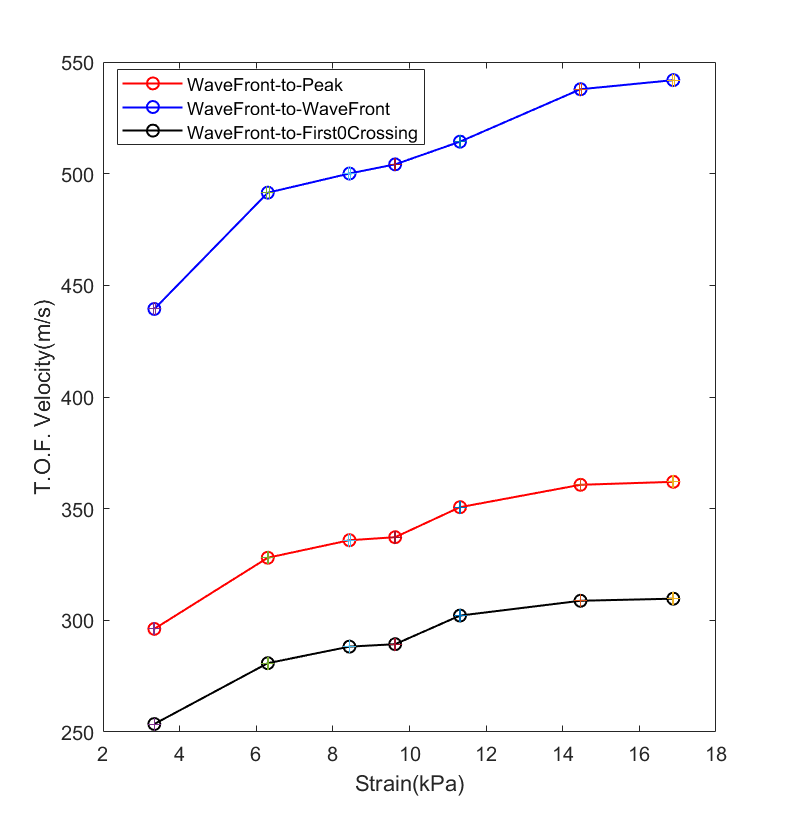
\includegraphics[height=7cm]{figures/2_strain_vs_velocity_20mm_1.png}}
  \hspace{1cm}
  \bisubcaptionbox{双对数处理后的应力 $P$ 与声速 $V_{\text{T.O.F.}}$ 的关系及其线性拟合}%
                  {Relationship between stress $P$ and sound velocity $V_{\text{T.O.F.}}$ after double logarithmic  and its linear fit}%
                  [6.4cm]{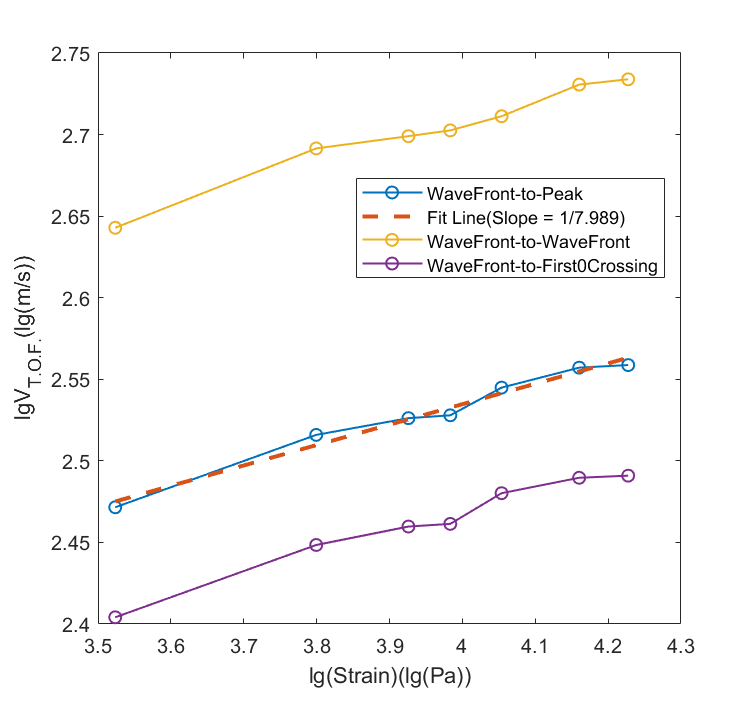
\includegraphics[height=7cm]{figures/2_strain_vs_velocity_20mm_2.png}}
  \bicaption{声速 $V_{\text{T.O.F.}}$ 与单轴应力 $P$ 的幂律关系。$P =$ \numlist{0.40;3.34;6.30;8.43;9.63;11.31;14.46}\unit{\kilo\pascal},颗粒介质为厚度 $L =19$\unit{\milli\meter} 的直径 $2$\unit{\milli\meter} 钢珠随机密堆积}
                  {Power-law relationship between the sound velocity $V_{\text{T.O.F.}}$ and the uniaxial stress $P$. $P =$ \numlist[
                    list-final-separator = { and }
                  ]{0.40;3.34;6.30;8.43;9.63;11.31;14.46}\unit{\kilo\pascal}, where the granular medium is a random close packing with steel beads of diameter $2\unit{\milli\meter}$ and thickness $L = 19$\unit{\milli\meter}}
  \label{fig:normalized_width_versus_P}
\end{figure}

由此可见,在我们的实验中,声速与单轴应力的指数关系实际上为 $V\propto p^{1/7.989}$。这一结果与等效介质理论的预言有较大的出入,这可能是因为 EMT 的假设条件对于颗粒物质实际上是相当苛刻的。可能的偏差原因如下:

\begin{enumerate}
  \item 真实的颗粒介质是异质性的。EMT 尝试通过增加颗粒系统的尺度与数量使得介质在统计上呈现各向同性,而在我们的实验中颗粒介质的约化厚度(Reduced Thickness)$L/d$ 并不高,约为 $7.33$;如果要在实验中做到这一点,那么作为探针的小振幅声波会因为颗粒介质因为尺度增加而增强的耗散性而剧烈衰减,使得响应信号的信噪比迅速降低。增加信号发生器的源振幅从而间接增加信噪比也是不可行的,因为在后文我们将讲述有关有限振幅波传播如何诱导颗粒介质内部接触与应力结构发生变化,即试探信号应当满足小振幅条件而不对颗粒介质造成泵浦效应;
  \item 颗粒介质中颗粒的接触在其表面并不一定是均匀分布的。有实验和计算证明,对受循环剪切的颗粒介质进行 X 射线旋转扫描建模追踪,对于 $D=12\unit{\milli\meter}$ 的示踪颗粒,其上下平均接触数分别为 $8.41$、$6.56$\cite{doi:10.1126/sciadv.abe8737}。由此可见,EMT 论述过程中所需求的“接触点在单个颗粒表面呈现均匀分布”,在大多数情况下都是并不严格的假设;
  \item 有效应力(effective pressure/stress)过低。在颗粒物理的研究中,对于有效应力的理解和定义多样,如使用体积模量的压强量纲来对应力进行重标定\cite{chengReviewAnalysisGranular2019}。在这里我们 Johnson 等人的表述,即借助标准大气压来定义有效应力: $P_{\text{eff}} = P - 1\unit{atm}$\cite{johnson_nonlinear_2005}。在这一标准下,不难发现在我们的实验中,颗粒介质的有效应力并不高(甚至有时是负数);而在成功重复出 EMT 预言的相关实验中,所施加应力往往都是 $\unit{\mega\pascal}$ 量级。既然声信号的传播可以粗糙理解为振动在颗粒介质内部力链上的传递,那么充分大的应力有助于颗粒介质的接触力更有效,响应信号的信噪比也会进一步提升。
\end{enumerate}

以上种种原因,使得在实验中重现 EMT 的各类假设是存在一定门槛的。因此以我们当前能达成的实验条件,测量出的声速与应力的指数关系与 EMT 的不符合也在理解范围以内。

%%% 可能是因为容器几何因素导致的 Yassen Effect,导致应力并不充分地施加到颗粒介质上。

\section{超声脉冲在颗粒介质中的展宽}
%%%%%%%%%%% 2024.04.26


颗粒介质通过异质性的力链网络传递应力,因此声波在颗粒介质中传播时会因为其非线性出现剧烈的畸变现象,其中脉冲超声波的展宽是较为明显的现象之一。本节讨论了颗粒介质厚度 $L$ 以及单轴应力 $P$ 对于脉冲波展宽的影响。

\subsection{归一化宽度的定义}

在数字信号处理中,常见的对于峰宽度的定义是峰的半高宽,例如在光谱分析中借助峰的半高宽定义的展宽来研究 Dopler 展宽、Stark 展宽等机制;事实上,前文中我们在处理响应信号的到达时间时,用于控制寻峰算法的参数中也的确包含了半高宽阈值,以此排除响应信号中固有的热噪声干扰。而在本小节中,我们引入的归一化宽度参数 $W$ 同时考虑了峰值与波前在时域中位置:

\begin{equation}
  W \equiv \frac{t_{1}-t_{0}}{t_{1}},
\end{equation}

其中 $t_{0}$ 与 $t_{1}$ 分别为波前与峰值的到达时间。我们在测定最佳信号参考点的时候已经能意识到,各个参考点出现的分离现象,即脉冲在传播距离上的展宽已经在一定程度上反映了“在颗粒介质中存在着较明显的色散关系”这一事实;而首峰到达时间 $t_{1}$ 定义的飞行时间速度,在距离上更具有稳定性。因此,通过与中心频率(这里指所发射的试探信号的频率 $f_{c}$)关联的 $t_{1}$ 来对信号进行缩放操作是合理的。后文通过数据处理后得到的图~\ref{fig:reference_point} 以及对应讨论中进一步证明这一点。

\subsection{归一化宽度与颗粒介质厚度的关系}

\subsubsection{理论推导}

为了理解归一化宽度的物理含义,我们先从最简单的一维弹簧链开始推导。在凝聚态物理课程中,我们已经学习了一维晶格的色散关系为

%%% 找一下基泰尔的citation

\begin{equation}
  \omega=\sqrt{\frac{4C}{M}}\left|\sin\left(\frac{ka}{2}\right)\right|,
\end{equation}

其中 $C$ 是弹簧的劲度系数,$M$ 是弹簧所连接质点的质量,$a$ 为平衡位置下的质点间距(晶格常数)。我们将其写为反函数形式:

\begin{equation}
  k(\omega) = \frac{2}{a}\arcsin{\left(\sqrt{\frac{M}{4C}}\omega\right)}.\label{eq:1D_dispersion_relation}
\end{equation}

为了求得此模型中的波传播速度 $V$,我们对式~\eqref{eq:1D_dispersion_relation} 应用长波极限,即 $ka\ll 1$:

\begin{equation}
  V = \lim_{ka\ll 1}\frac{\omega}{k} = \sqrt{\frac{C}{M}}a.
\end{equation}

使用 $V$ 替换式~\eqref{eq:1D_dispersion_relation} 中的 $C$,$M$ 项,且假定长波极限下的声速 $V$ 充分大,使得我们足以通过 Maclaurin 级数将波矢项 $k(\omega)$ 展开至前两项:

\begin{equation}
  k = \frac{2}{a}\left[\frac{a\omega}{2V} + \frac{1}{6}\left(\frac{a\omega}{2V}\right)^{3} + o\left(\frac{1}{V^3}\right)\right]\approx\frac{\omega}{V} + \frac{2\omega^{3}a^{2}}{3V^{3}}+o(\omega^{3}),
\end{equation}

将其代入至波数项中,我们将看到

\begin{equation}
  \text{exp}\left[{\ii \left(\frac{\omega}{V} + \frac{2a^{2}\omega^{3}}{3V^{3}}\right)x}\right] = \text{exp}[{\ii\omega t_{1}}]\text{exp}\left[{\ii\left(\frac{\omega}{\omega_{1}}\right)^{3}}\right],\quad t_{1} = \frac{x}{V},\quad \omega_{1} = \sqrt[3]{\frac{3V^{3}}{2a^{2}x}}.\label{eq:rescale_method}
\end{equation}

而我们已经知道,在傅里叶变换中,存在关系

\begin{align}
  \mathcal{F}[f(t+t_{1})] = \mathcal{F}[f(t)]{\ee}^{\ii\omega t_{1}},\label{eq:translation_property}\\
  \mathcal{F}[f(\omega_{1}t)] = \frac{1}{|\omega_{1}|}\hat{f}\left(\frac{\omega}{\omega_{1}}\right),\label{eq:scale_property}\\
  \mathcal{F}[\text{Ai}(t)] = \text{exp}\left[\ii\cdot \frac{1}{3}\omega^3\right].
\end{align}

其中 $\text{Ai}(t)$ 是 Airy 函数。将波数项代入至 $a(x,-t)$ 中,并对其进行傅里叶变换:

\begin{equation}
  \mathcal{F}[a(x,-t)] = \int_{-\infty}^{+\infty}A_{0}{\ee}^{\ii\omega t_{1}}{\ee}^{\ii(\omega/\omega_{1})^{3}}e^{\ii\omega t}e^{-\ii\omega t}\mathrm{d}t = A_{0}{\ee}^{\ii\omega t_{1}}{\ee}^{\ii(\omega/\omega_{1})^{3}}.
\end{equation}

所以,根据傅里叶变换的平移性质~\eqref{eq:translation_property}与尺度放缩性质~\eqref{eq:scale_property},我们得到经由颗粒介质传播的响应信号形式可近似为通过 $\omega_{1}$ 控制峰宽度的 Airy 函数:

\begin{equation}
  s(x,t) = \omega_{1}\text{Ai}\left[\omega_{1}(t_{1}-t)\right].
\end{equation}

因此,在一维弹簧链中,脉冲波传播到距离 $L$ 处的归一化宽度 $W$ 为

\begin{equation}
  W \approx \frac{\pi}{2\omega_{1}}\frac{1}{t_{1}}\propto L^{-2/3}.
\end{equation}

考虑一维球链时,使用 $a=2R$ 替换即可得到对应的公式\cite{PhysRevE.91.022205}。接下来我们进一步考虑颗粒介质中衰减项 $\alpha$ 的影响。引入弹性模量的涨落 $\nu_{K} = \Delta K^{-1}/\bar{K}^{-1}$ 与对应的关联长度 $L_{c}$,我们可以得到一维随机层理论对于衰减项的描述:

\begin{equation}
  \alpha(\omega) = k^{\prime\prime}(\omega) = [\sigma_{K}^{2}L_{c}^{n-1}]\left(\frac{\omega}{V}\right)^{n}.
\end{equation}

其中满足

\begin{align}
  V &= \bar{V} = \sqrt{\frac{\bar{K}}{\bar{\rho}}},\\
  \gamma &= \int_{0}^{+\infty}\langle\nu_{K}(0)\nu_{K}(x)\rangle\mathrm{d}x = \sigma_{K}^{2}L_{c}.
\end{align}

通过引入虚波矢 $k^{\prime\prime}$ 写出频域内的信号分布,并仿照上面一维弹簧链中的式~\eqref{eq:rescale_method} 进行缩放操作:

\begin{equation}
  \widetilde{a}(\omega) = {\ee}^{ik^{\prime}x}e^{-k^{\prime\prime}x} = e^{i\omega t_{1}}e^{-\left(\frac{\omega}{\omega_{1}}\right)^{n}},\quad t_{1} = \frac{x}{V},\quad \omega_{1} = \sqrt[n]{\frac{V^{n}}{\sigma_{K}^{2}L_{c}^{n-1}x}}.
\end{equation}

因此得到归一化宽度:

\begin{equation}
W\sim \frac{1}{\omega_{1}t_{1}} = (\sigma_{K})^{\frac{2}{n}}\left(\frac{L_{c}}{x}\right)^{\frac{n-1}{n}}
\end{equation}

在一维随机分层介质中有 $n=2$, 因此在 $x = L$ 处归一化宽度为

\begin{equation}
  W\propto L^{-\frac{1}{2}}.
\end{equation}

由此我们得到了同时考虑了色散关系与衰减项的归一化宽度与颗粒介质厚度之间的指数关系。

\subsubsection{实验验证}

我们设定 $5$ 循环 $30\unit{\kilo\Hz}$、振幅为 $1\unit{VPP}$ 的连续正弦波列电压模拟信号作为试探信号的激励源,使用颗粒为直径 $2\unit{\milli\meter}$ 的钢珠生成随机密堆积,施加的单轴应力为 $9\unit{\kilo\Pa}$;每一厚度都各自单独重新制备 7 次随机密堆积以尽可能消除实验误差,分别测定了颗粒介质厚度为 $\numlist{6;11;16;20;24;30}\unit{\milli\metre}$ 时的响应信号,并且对各到达时间的数据进行系综平均,计算其标准差作为误差。图~\ref{fig:reference_point} 展示了其中一组响应信号的图像,其幅值通过相干首波峰值 $A_{1}$ 进行归一化处理,且时间轴以首峰到达时间 $t_{1}$ 进行重标定放缩:

\begin{figure}[!htp]
  \centering
  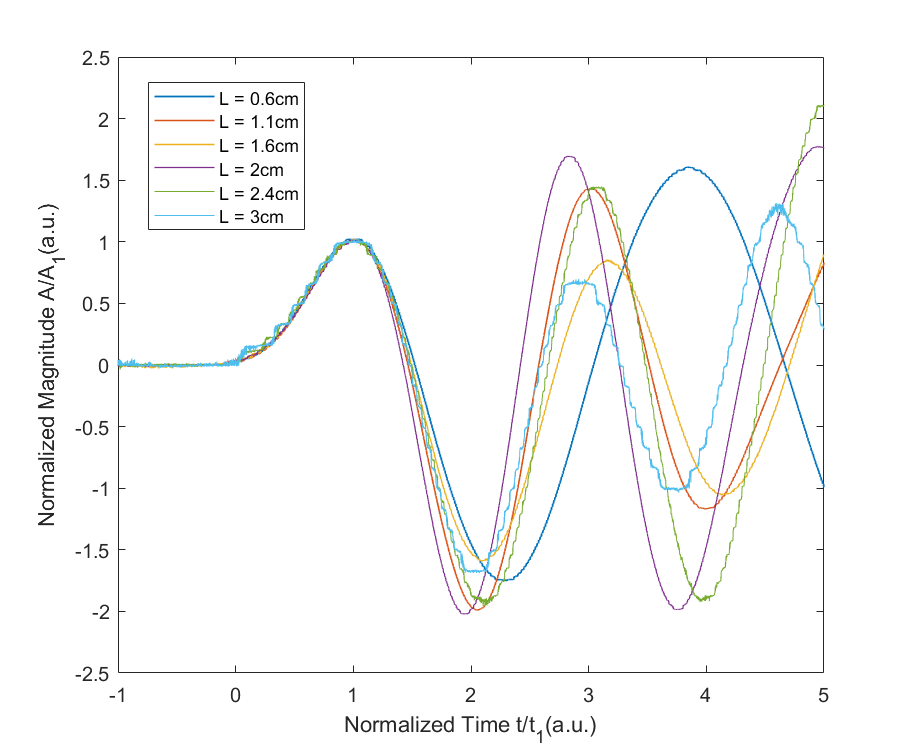
\includegraphics[height=6cm]{2_Rescaled_Magnitude_differing_in_Distance.png}
  \bicaption{通过相干波峰 $A_{1}$ 归一化,且时间轴以波峰到达时间 $t_{1}$ 进行缩放后的不同颗粒样品厚度下测得的响应信号}{Response signal captured at different granular sample thicknesses, normalized with coherent wave peak $A_{1}$ and time axis rescaled with peak arrival time $t_{1}$}
  \label{fig:reference_point}
\end{figure}

可以发现,虽然采集信号时的颗粒介质厚度各异,但是通过幅值归一化与时间轴的缩放,仍能够观察到“响应信号可以提取出相干首波”的本质特征。当 $t/t_{1} > 1$,响应信号的宽度开始出现显著变化;而在前面的信号参考点选取的实验中,我们已经知道,$t_{1}$ 是一个性质较为良好的参考点,因此我们可以通过借助 $t_{1}$ 定义的归一化宽度 $W$ 来探究其与颗粒介质厚度,即信号传播距离 $L$ 之间的关系。

图~\ref{fig:normalized_width_versus_L} 展示了上述实验中测得的归一化宽度 $W$ 与颗粒介质厚度 $L$ 之间的关系。为了观察两者之间是否存在指数关系,对图像使用了双对数处理,并对其数据点进行了线性拟合求得斜率。不难看出,我们得出的结果约为 $W\propto L^{-0.448}$,与理论推导的 $W\propto L^{-1/2}$ 已经相当接近。

需要说明的是,这种偏差存在两种来源:

\begin{enumerate}
  \item 波前到达时间的选取并不是绝对的。既然我们是通过 $S(t_{0}) = A_{1}\cdot k$($k\in(0,0.1]$)确定的 $t_{0}$,那么 $k$ 的具体数值会影响到 $t_{0}$ 的选取,从而影响到归一化宽度 $W$ 的测定;而在传播距离较大时,响应信号的信噪比会因为颗粒介质吸收、耗散引起的衰减而急剧降低,若要对经由任意传播距离的响应信号划定一条共通可行的 $k$ 实际上是并不容易的。在真实实验以及后续的数据处理时,$k$ 的具体数值需要通过经验来调整,使得归一化宽度的测定并不严格;
  \item 理论推导中的 $n=2$ 是一维随机分层介质的情况。虽然我们已经将色散关系和衰减同时纳入考虑,并且实验模式中超声波的传播偏向于柱坐标中单个 $z$ 轴方向上,但是这一切仍不能改变“实际的颗粒介质仍然是三维体系”的事实,因此出现 $-0.448\sim-1/2$ 的偏差仍然是在理解范围内的。
\end{enumerate}

\begin{figure}[!hbtp]
  \centering
  \bisubcaptionbox{相干首波峰宽度 $t_{1} - t_{0}$}%
                  {Coherent wave peak width $t_{1} - t_{0}$}%
                  [6.4cm]{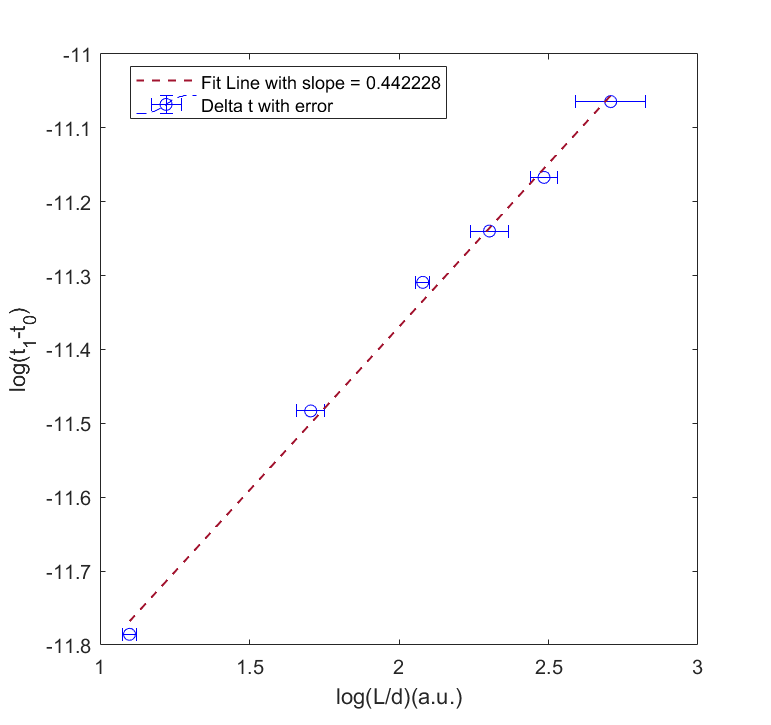
\includegraphics[height=7cm]{figures/2_t1-t0_L.png}}
  \hspace{1cm}
  \bisubcaptionbox{相干首波归一化宽度 $W$}%
                  {Coherent first wave normalized width $W$}%
                  [6.4cm]{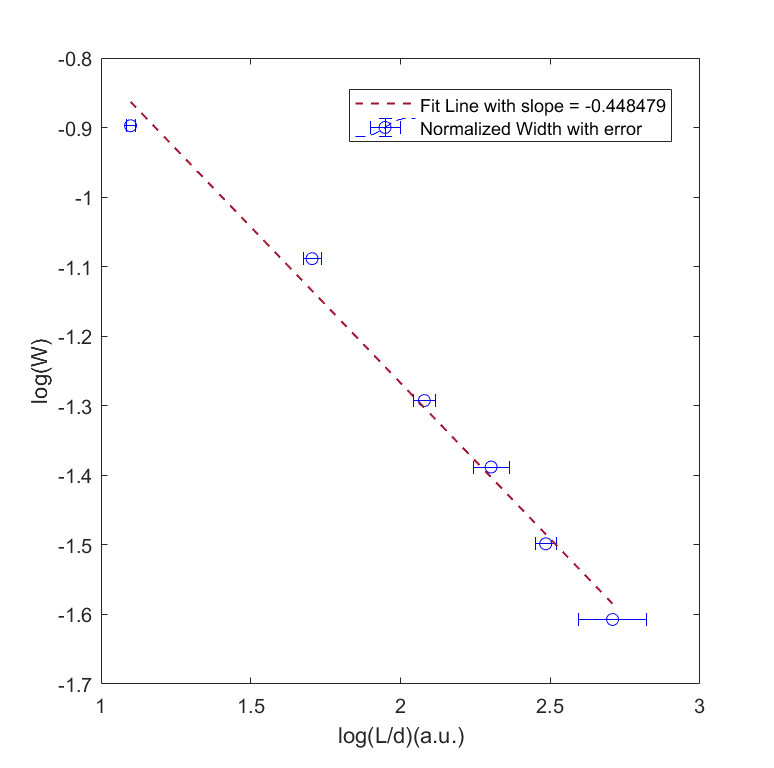
\includegraphics[height=7cm]{figures/2_W_L.png}}
  \bicaption{颗粒介质厚度为 \numlist{6;11;16;20;24;30} \unit{\milli\metre} 时的响应信号首峰宽度 $t_{1} - t_{0}$ 与归一化宽度 $W$}
                  {First peak width $t_{1} - t_{0}$ and normalized width $W$ of response signal at granular medium thickness of \numlist[
                    list-final-separator = { and }
                  ]{6;11;16;20;24;30} \unit{\milli\metre}}
  \label{fig:normalized_width_versus_L}
\end{figure}

\subsection{归一化宽度与单轴应力的关系}

类似于上述实验中考虑的颗粒介质厚度,即脉冲传播距离 $L$ 对脉冲归一化宽度 $W$ 的影响,我们也对在不同单轴应力 $P$ 下的归一化宽度 $W(P)$ 进行了计算与绘图,数据来自于小节~\ref{sec:stress_velocity_relation} 中单轴应力与声速关系的实验。但遗憾的是,如图~\ref{fig:normalized_width_versus_P} 所示,我们没有观察到两者之间存在着任何明显的规律。

\begin{figure}[!hbtp]
  \centering
  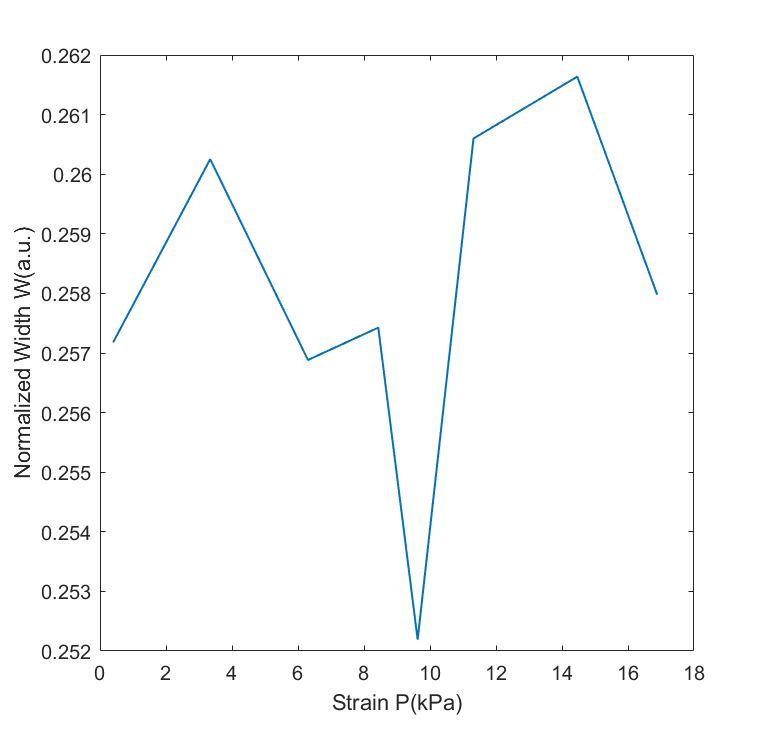
\includegraphics[height=7cm]{figures/2_W_norm&Strain.png}
  \bicaption{单轴应力 $P$ 与归一化宽度 $W$ 的关系}{Relationship between uniaxial stress $P$ and normalized width $W$}
  \label{fig:normalized_width_versus_P}
\end{figure}

目前对于该现象的解释是,颗粒介质中本身存在着如 Jassen Effect 等现象,即在诸如圆筒形容器中颗粒介质所受重力并非完全沿轴向传递,而是会有一部分力被颗粒介质中的结构分配到径向。这与寻常的连续介质所产生的液压规律 $p=\rho gh$ 完全不同,因此早期人类的粮仓会因为设计不合理而被过量的径向应力破坏而坍塌\cite{sperlExperimentsCornPressure2006}。在我们的实验中,由于容器的几何因素,可能类似的效应使得颗粒介质对于脉冲信号的响应规律性受到影响,导致所观察到的 $W(P)$ 与 $P$ 之间的关系并不明显。